%!TEX root=../protocol.tex	% Optional

\section{Zadání}
\subsection{Úvod}
Metalická vedení jsou nejčastěji používanou variantou fyzické vrstvy komunikačního kanálu. Při použití je nutno
uvažovat jejich vlastnosti jako dlouhého vedení, tzn. respektovat konečnou rychlost šíření elektromagnetických
vln a potřebu impedančního přizpůsobení.
\subsection{Postup měření}
V rámci měření se nejprve seznámíte s nastavením impulsního generátoru, který poté spolu s osciloskopem
využijete pro studium šíření číslicových signálů metalickým vedením.
\subsection{Impulsní generátor}
Seznamte se s ovládáním impulsního generátoru (nastavení periody, střídy, rychlosti hran), průběhy zobrazte
na osciloskopu. Na generátoru nastavte pulsy s šířkou 150 – 200 ns, periodou cca 2 ms a maximální rychlostí
hrany.
\begin{figure}[h]
\centering
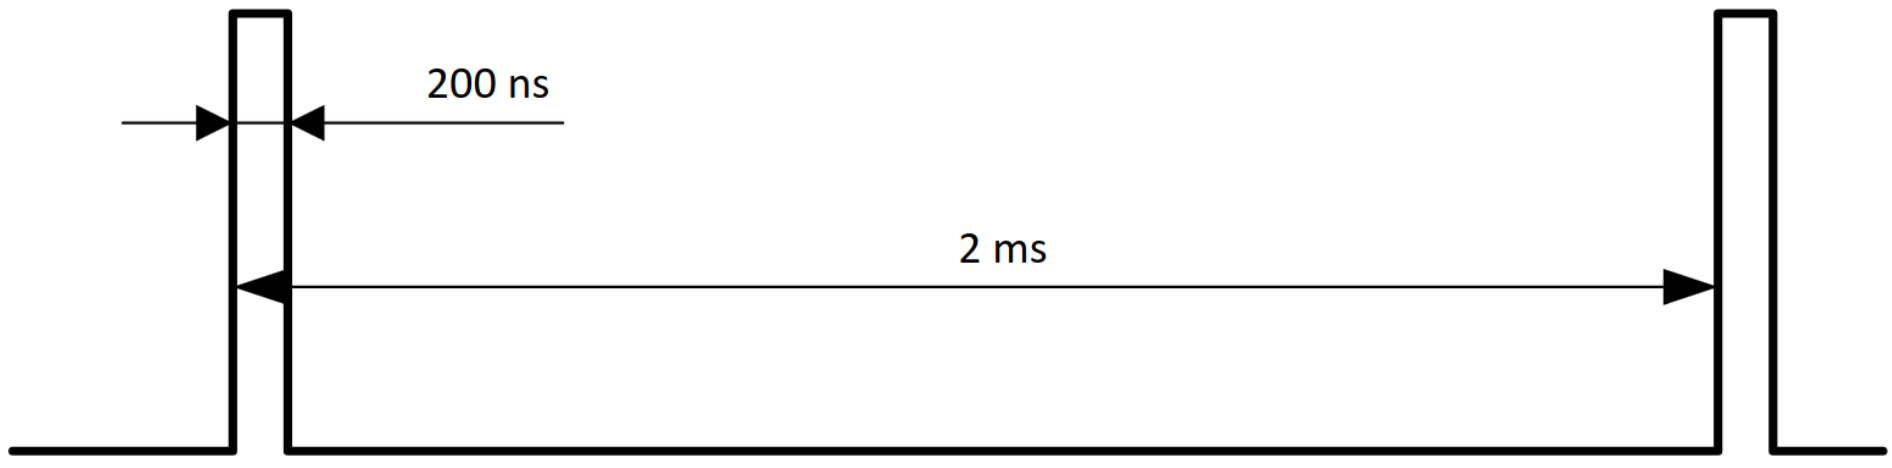
\includegraphics[width=12cm]{images/01-zadani.png}
\caption{Generovaný signál}
\label{fig:1}
\end{figure}
\subsection{Činitel odrazu na konci vedení}
Definujte činitel odrazu na konci vedení a určete jeho hodnoty pro koaxiální kabel s charakteristickou
impedancí 50 $\Omega$, pokud je zakončen impedancemi 0 $\Omega$, 25 $\Omega$, 50 $\Omega$, 100 $\Omega$ a $\infty$ $\Omega$.
\newpage
\subsection{Reflektometrické měření délky vedení}
Pomocí osciloskopu a generátoru změřte délku předloženého „dlouhého“ koaxiálního kabelu. Rychlost šíření
signálu kabelem je 0,65 násobek rychlosti světla ve vakuu. Vysvětlete princip měření a uveďte, jakou základní
podmínku musíte splnit, aby měření bylo principiálně možné?\\\\
Osciloskop a začátek kabelového vedení připojte paralelně k výstupu generátoru. Konec vedení můžete připojit
na druhý kanál osciloskopu.
\begin{figure}[h]
\centering
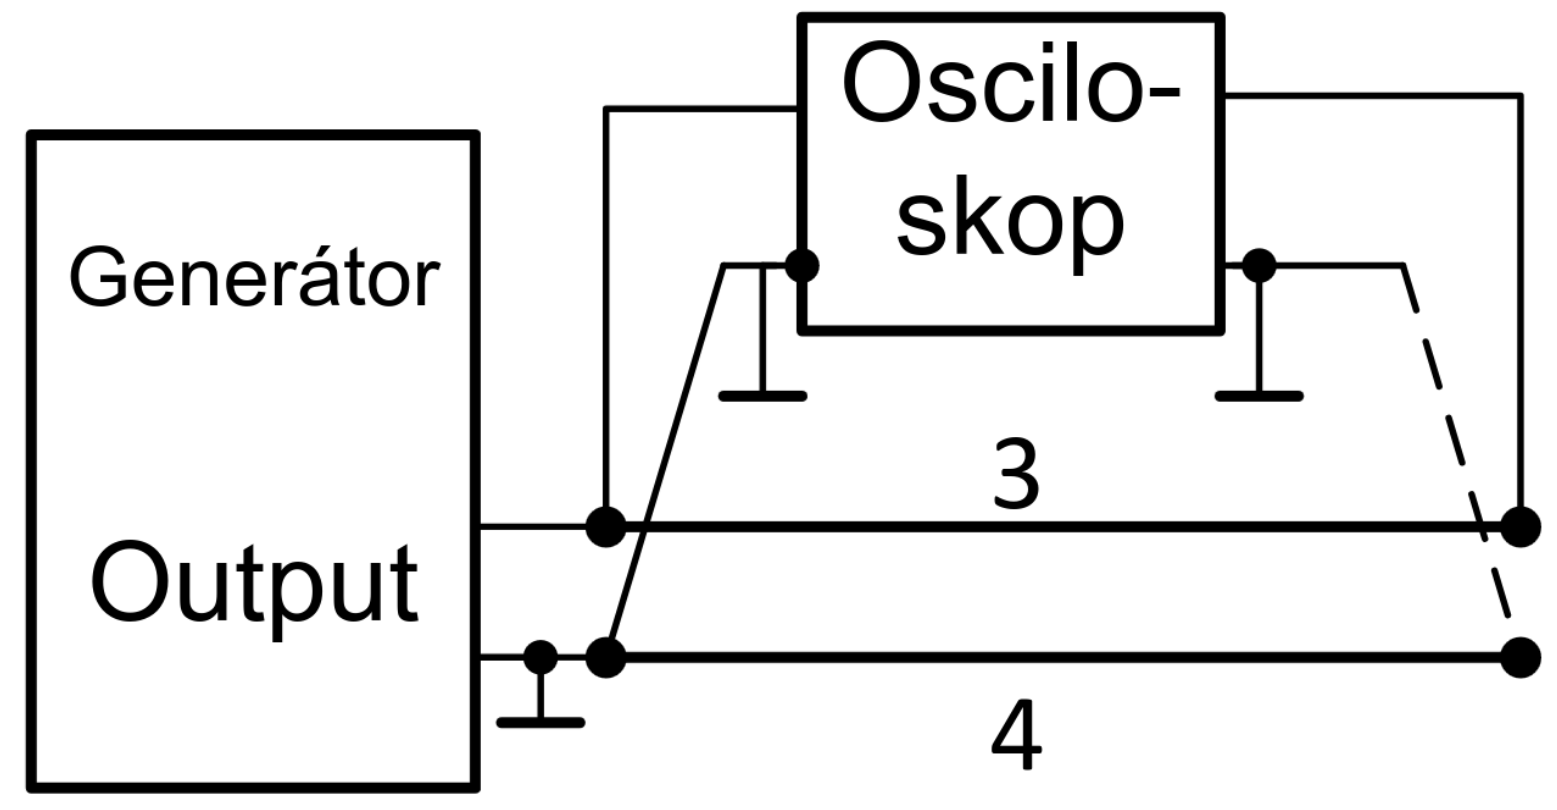
\includegraphics[width=12cm]{images/02-zadani.png}
\caption{Uspořádání pro měření délky kabelu}
\label{fig:2}
\end{figure}
\subsection{Měření charakteristické impedance vedení}
Ověřte hodnotu charakteristické impedance předloženého koaxiálního kabelu. Na konec kabelu připojte
nastavitelný rezistor $R_Z$ a nastavte hodnotu, při níž nedochází k odrazu. Multimetrem pak změřte hodnotu jeho
odporu.
\begin{figure}[h]
\centering
\includegraphics[width=12cm]{images/03-zadani.png}
\caption{Uspořádání pro měření impedance vedení}
\label{fig:3}
\end{figure}
\subsection{Impedanční přizpůsobení na počátku vedení}
Demonstrujte metodu přizpůsobení vedení na jeho počátku. Vedení připojené ke generátoru je na vstupu
impedančně přizpůsobeno, neboť výstupní impedance generátoru je 50 $\Omega$. Konec vedení ponechte
nepřizpůsobený – 1 M$\Omega$ vstupní impedance osciloskopu. Na generátoru nastavte délku pulsu alespoň na 100 $\mu$s
a pozorujte průběhy (speciálně hrany pulsů v časovém detailu) na počátku i na konci vedení. Průběh na počátku
vedení vysvětlete.
\subsection{Dodatečné informace}
U všech měření je třeba dbát na to, aby vstupní impedance osciloskopu byla 1 M$\Omega$, nikoliv 50 $\Omega$.
\subsection{Šíření signálu v bezeztrátovém vedení}
\begin{figure}[h]
\centering
\includegraphics[width=15cm]{images/04-zadani.png}
\caption{}
\label{fig:4}
\end{figure}